\documentclass[12pt]{article}
\usepackage[margin=2cm]{geometry}
\usepackage{amsmath}
\usepackage{slashed}
\usepackage{tikz}

\begin{document}

\noindent
Moller scattering is the result of interactions between electrons.
The following diagram shows the geometry of a typical collider experiment
that generates Moller scattering data.
\begin{center}
\begin{tikzpicture}
\draw[dashed] (0,0) circle (0.5cm);
\draw[thick,->] (2,0) node[anchor=west] {$e^-$} -- (0.6,0);
\draw[thick,->] (-2,0) node[anchor=east] {$e^-$} -- (-0.6,0);
\draw[thick,->] (0.40,0.40) -- (1.3,1.3) node[anchor=south west] {$e^-$};
\draw[thick,->] (-0.4,-0.4) -- (-1.3,-1.3) node[anchor=north east] {$e^-$};
\draw (1,0.5) node {$\theta$};
\end{tikzpicture}
\end{center}

\noindent
Here is the same diagram with momentum and spinor labels.

\begin{center}
\begin{tikzpicture}
\draw[dashed] (0,0) circle (0.5cm);
\draw[thick,->] (2,0) node[anchor=west] {$p_2, u_2$} -- (0.6,0);
\draw[thick,->] (-2,0) node[anchor=east] {$p_1, u_1$} -- (-0.6,0);
\draw[thick,->] (0.40,0.40) -- (1.3,1.3) node[anchor=south west] {$p_3, u_3$};
\draw[thick,->] (-0.4,-0.4) -- (-1.3,-1.3) node[anchor=north east] {$p_4, u_4$};
\draw (1,0.5) node {$\theta$};
\end{tikzpicture}
\end{center}

\noindent
In center of mass coordinates the momentum vectors are
$$
p_1=\begin{pmatrix}E\\0\\0\\p\end{pmatrix}\quad
p_2=\begin{pmatrix}E\\0\\0\\-p\end{pmatrix}\quad
p_3=\begin{pmatrix}
E\\
p\sin\theta\cos\phi\\
p\sin\theta\sin\phi\\
p\cos\theta
\end{pmatrix}
\quad
p_4=\begin{pmatrix}
E\\
-p\sin\theta\cos\phi\\
-p\sin\theta\sin\phi\\
-p\cos\theta
\end{pmatrix}
$$

\noindent
where $E=\sqrt{p^2+m^2}$.

\bigskip
\noindent
The spinors are
\begin{gather*}
\underset{\text{inbound electron, spin up}}
{u_{11}=\begin{pmatrix}E+m\\0\\p\\0\end{pmatrix}}
\quad
\underset{\text{inbound electron, spin down}}
{u_{12}=\begin{pmatrix}0\\E+m\\0\\-p\end{pmatrix}}
\quad
\underset{\text{inbound electron, spin up}}
{u_{21}=\begin{pmatrix}E+m\\0\\-p\\0\end{pmatrix}}
\quad
\underset{\text{inbound electron, spin down}}
{u_{22}=\begin{pmatrix}0\\E+m\\0\\p\end{pmatrix}}
\\
\underset{\text{outbound electron, spin up}}
{u_{31}=\begin{pmatrix}E+m\\0\\p_{3z}\\p_{3x}+ip_{3y}\end{pmatrix}}
\quad
\underset{\text{outbound electron, spin down}}
{u_{32}=\begin{pmatrix}0\\E+m\\p_{3x}-ip_{3y}\\-p_{3z}\end{pmatrix}}
\quad
\underset{\text{outbound electron, spin up}}
{u_{41}=\begin{pmatrix}E+m\\0\\p_{4z}\\p_{4x}+ip_{4y}\end{pmatrix}}
\quad
\underset{\text{outbound electron, spin down}}
{u_{42}=\begin{pmatrix}0\\E+m\\p_{4x}-ip_{4y}\\-p_{4z}\end{pmatrix}}
\end{gather*}

\noindent
The spinors shown above are not individually normalized.
Instead, a combined spinor normalization constant
$N=(E+m)^4$ will be used.

\bigskip
\noindent
The following formula computes a probability density $|\mathcal{M}_{abcd}|^2$
for Moller scattering where the subscripts $abcd$ are the spin states of the electrons.
\begin{equation*}
|\mathcal{M}_{abcd}|^2=\frac{e^4}{N}
\left|
\frac{1}{t}(\bar{u}_{3c}\gamma^\mu u_{1a})(\bar{u}_{4d}\gamma_\mu u_{2b})
-\frac{1}{u}(\bar{u}_{4d}\gamma^\nu u_{1a})(\bar{u}_{3c}\gamma_\nu u_{2b})
\right|^2
\end{equation*}

\noindent
Symbol $e$ is electron charge.
Symbols $t$ and $u$ are Mandelstam variables $t=(p_1-p_3)^2$ and $u=(p_1-p_4)^2$.

\bigskip
\noindent
Let
\begin{equation*}
a_1=(\bar{u}_{3c}\gamma^\mu u_{1a})(\bar{u}_{4d}\gamma_\mu u_{2b})
\qquad
a_2=(\bar{u}_{4d}\gamma^\nu u_{1a})(\bar{u}_{3c}\gamma_\nu u_{2b})
\end{equation*}

\noindent
Then
\begin{align*}
|\mathcal{M}_{abcd}|^2
&=
\frac{e^4}{N}
\left|\frac{a_1}{t} - \frac{a_2}{u}\right|^2\\
&=
\frac{e^4}{N}
\left(\frac{a_1}{t} - \frac{a_2}{u}\right)\left(\frac{a_1}{t} - \frac{a_2}{u}\right)^*\\
&=
\frac{e^4}{N}
\left(
\frac{a_1a_1^*}{t^2} - \frac{a_1a_2^*}{tu} -
\frac{a_1^*a_2}{tu} + \frac{a_2a_2^*}{u^2}
\right)
\end{align*}

\noindent
The expected probability density $\langle|\mathcal{M}|^2\rangle$ is computed by
summing $|\mathcal{M}_{abcd}|^2$ over all spin states and dividing by the number
of inbound states.
There are four inbound states.
\begin{align*}
\langle|\mathcal{M}|^2\rangle
&=
\frac{1}{4}\sum_{a=1}^2\sum_{b=1}^2\sum_{c=1}^2\sum_{d=1}^2
|\mathcal{M}_{abcd}|^2\\
&=
\frac{e^4}{4N}\sum_{a=1}^2\sum_{b=1}^2\sum_{c=1}^2\sum_{d=1}^2
\left(
\frac{a_1a_1^*}{t^2}-\frac{a_1a_2^*}{tu}-\frac{a_1^*a_2}{tu}+\frac{a_2a_2^*}{u^2}
\right)
\end{align*}

\noindent
Use the Casimir trick to replace sums over spins with matrix products.
\begin{align*}
f_{11}&=\frac{1}{N}\sum_{abcd}a_1a_1^*=
\mathop{\rm Tr}\left(
(\slashed{p}_3+m)\gamma^\mu(\slashed{p}_1+m)\gamma^\nu
\right)
\mathop{\rm Tr}\left(
(\slashed{p}_4+m)\gamma_\mu(\slashed{p}_2+m)\gamma_\nu
\right)
\\
f_{12}&=\frac{1}{N}\sum_{abcd}a_1a_2^*=
\mathop{\rm Tr}\left(
(\slashed{p}_3+m)\gamma^\mu(\slashed{p}_1+m)\gamma^\nu
(\slashed{p}_4+m)\gamma_\mu(\slashed{p}_2+m)\gamma_\nu
\right)
\\
f_{22}&=\frac{1}{N}\sum_{abcd}a_2a_2^*=
\mathop{\rm Tr}\left(
(\slashed{p}_4+m)\gamma^\mu(\slashed{p}_1+m)\gamma^\nu
\right)
\mathop{\rm Tr}\left(
(\slashed{p}_3+m)\gamma_\mu(\slashed{p}_2+m)\gamma_\nu
\right)
\end{align*}

\noindent
Hence
\begin{equation*}
\langle|\mathcal{M}|^2\rangle
=\frac{e^4}{4}
\left(
\frac{f_{11}}{t^2}-\frac{f_{12}}{tu}-\frac{f_{12}^*}{tu}+\frac{f_{22}}{u^2}
\right)
\end{equation*}

\noindent
Run ``moller-scattering-1.txt'' to verify the Casimir trick.

\bigskip
\noindent
The following momentum formulas are equivalent to the Casimir trick.
(Recall that $a\cdot b=a^\mu g_{\mu\nu}b^\nu$)
\begin{align*}
f_{11}&=
32 (p_1\cdot p_2) (p_3\cdot p_4) +
32 (p_1\cdot p_4) (p_2\cdot p_3) -
32 m^2 (p_1\cdot p_3) -
32 m^2 (p_2\cdot p_4) +
64 m^4
\\
f_{12}&=
-32 (p_1\cdot p_2) (p_3\cdot p_4)
+ 16 m^2 (p_1\cdot p_2) + 16 m^2 (p_1\cdot p_3) + 16 m^2 (p_1\cdot p_4) \\
&\phantom{=}\qquad{} + 16 m^2 (p_2\cdot p_3) + 16 m^2 (p_2\cdot p_4) + 16 m^2 (p_3\cdot p_4) - 32 m^4
\\
f_{22}&=
32 (p_1\cdot p_2) (p_3\cdot p_4) +
32 (p_1\cdot p_3) (p_2\cdot p_4) -
32 m^2 (p_1\cdot p_4) -
32 m^2 (p_2\cdot p_3) +
64 m^4
\end{align*}

\noindent
In Mandelstam variables $s=(p_1+p_2)^2$, $t=(p_1-p_3)^2$, and $u=(p_1-p_4)^2$ the formulas are
\begin{align*}
f_{11} &= 8 s^2 + 8 u^2 - 64 s m^2 - 64 u m^2 + 192 m^4
\\
f_{12} &= -8 s^2 + 64 s m^2 - 96 m^4
\\
f_{22} &= 8 s^2 + 8 t^2 - 64 s m^2 - 64 t m^2 + 192 m^4
\end{align*}

\subsection*{High energy approximation}
When $E\gg m$ a useful approximation is to set $m=0$ and obtain
\begin{align*}
f_{11}&=8s^2+8u^2\\
f_{12}&=-8s^2\\
f_{22}&=8s^2+8t^2
\end{align*}

\noindent
For $m=0$ the Mandelstam variables are
\begin{align*}
s&=4E^2
\\
t&=-2E^2(1-\cos\theta)%=-4E^2\sin^2(\theta/2)
\\
u&=-2E^2(1+\cos\theta)%=-4E^2\cos^2(\theta/2)
\end{align*}

\noindent
It follows that
\begin{equation*}
t^2u^2=16E^8\sin^4\theta
\end{equation*}

\noindent
The corresponding expected probability density is
\begin{align*}
\langle|\mathcal{M}|^2\rangle
&=\frac{e^4}{4}
\left(
\frac{f_{11}}{t^2}-\frac{f_{12}}{tu}-\frac{f_{12}^*}{tu}+\frac{f_{22}}{u^2}
\right)
\\
&=\frac{e^4}{4t^2u^2}
\left(
u^2f_{11}-tuf_{12}-tuf_{12}^*+t^2f_{22}
\right)
\\
&=\frac{e^4}{4t^2u^2}
\left(
u^2\left(8s^2+8u^2\right)+16s^2tu+t^2\left(8s^2+8t^2\right)
\right)
\\
&=\frac{e^4}{64E^8\sin^4\theta}
\left(256 E^8\cos^4\theta+1536 E^8\cos^2\theta+2304 E^8\right)
\\
&=\frac{4e^4}{\sin^4\theta}
\left(\cos^4\theta+6\cos^2\theta+9\right)
\\
&=4e^4\frac{\left(\cos^2\theta+3\right)^2}{\sin^4\theta}
\end{align*}

\noindent
Run ``moller-scattering-2.txt'' to verify.

\subsection*{Cross section}
The differential cross section is
\begin{equation*}
\frac{d\sigma}{d\Omega}
=\frac{\langle|\mathcal{M}|^2\rangle}{64\pi^2s}
=\frac{e^4}{64\pi^2E^2}\,\frac{\left(\cos^2\theta+3\right)^2}{\sin^4\theta}
\end{equation*}

\noindent
Substituting $e^4=16\pi^2\alpha^2$ yields
\begin{equation*}
\frac{d\sigma}{d\Omega}=\frac{\alpha^2}{4E^2}\,\frac{\left(\cos^2\theta+3\right)^2}{\sin^4\theta}
\end{equation*}

\noindent
We can integrate $d\sigma$ to obtain a cumulative distribution function.
Recall that
\begin{equation*}
d\Omega=\sin\theta\,d\theta\,d\phi
\end{equation*}
Hence
\begin{equation*}
d\sigma=\frac{\alpha^2}{4E^2}\,\frac{\left(\cos^2\theta+3\right)^2}{\sin^4\theta}\sin\theta\,d\theta\,d\phi
\end{equation*}

\noindent
Let $I(\theta)$ be the following integral of $d\sigma$.
\begin{align*}
I(\theta)&=\left(\frac{4E^2}{\alpha^2}\right)\frac{1}{2\pi}\int_0^{2\pi}\int d\sigma
\\
&=\int\frac{\left(\cos^2\theta+3\right)^2}{\sin^4\theta}\sin\theta\,d\theta
\\
&=-\cos\theta-\frac{8\cos\theta}{\sin^2\theta},
\quad a\le\theta\le\pi-a
\end{align*}

\noindent
Angular support is limited to an arbitrary $a>0$ because $I(0)$ and $I(\pi)$ are undefined.

\bigskip
\noindent
Let $C$ be the normalization constant
\begin{equation*}
C=I(\pi-a)-I(a)
\end{equation*}

\noindent
Then the cumulative distribution function $F(\theta)$ is
\begin{equation*}
F(\theta)=\frac{I(\theta)-I(a)}{C},\quad a\le\theta\le\pi-a
\end{equation*}

\noindent
The probability of observing scattering events in the interval $\theta_1$ to $\theta_2$
can now be computed.
\begin{equation*}
P(\theta_1\le\theta\le\theta_2)=F(\theta_2)-F(\theta_1)
\end{equation*}

\noindent
Probability density function $f(\theta)$ is the derivative of $F(\theta)$.
\begin{equation*}
f(\theta)
=\frac{dF(\theta)}{d\theta}
=\frac{1}{C}\frac{\left(\cos^2\theta+3\right)^2}{\sin^4\theta}\sin\theta
\end{equation*}

\noindent
Run ``moller-scattering-3.txt'' to draw a graph of $f(\theta)$ for $a=\pi/6=30^\circ$.

\begin{center}
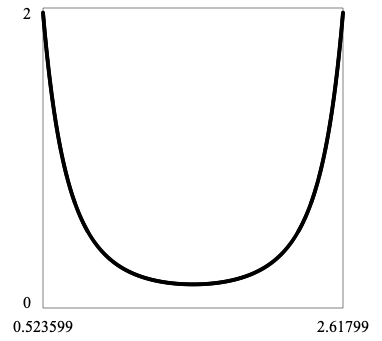
\includegraphics[scale=0.5]{moller-scattering.png}
\end{center}

\noindent
Probability distribution for $30^\circ$ bins ($a=30^\circ$).
\begin{center}
\begin{tabular}{|c|c|c|}
\hline
$\theta_1$ & $\theta_2$ & $P(\theta_1\le\theta\le\theta_2)$\\
\hline
$0^\circ$ & $30^\circ$ & -- \\
$30^\circ$ & $60^\circ$ & 0.40 \\
$60^\circ$ & $90^\circ$ & 0.10 \\
$90^\circ$ & $120^\circ$ & 0.10 \\
$120^\circ$ & $150^\circ$ & 0.40 \\
$150^\circ$ & $180^\circ$ & -- \\
\hline
\end{tabular}
\end{center}

\subsection*{Notes on Eigenmath scripts}
In component notation, the trace operators of the Casimir trick become sums over
a repeated index, in this case $\alpha$.
\begin{align*}
f_{11}&=
\left(
(\slashed{p}_3+m)^\alpha{}_\beta
\gamma^{\mu\beta}{}_\rho
(\slashed{p}_1+m)^\rho{}_\sigma
\gamma^{\nu\sigma}{}_\alpha
\right)
\left(
(\slashed{p}_4+m)^\alpha{}_\beta
\gamma_\mu{}^\beta{}_\rho
(\slashed{p}_2+m)^\rho{}_\sigma
\gamma_\nu{}^\sigma{}_\alpha
\right)
\\
f_{12}&=
(\slashed{p}_3+m)^\alpha{}_\beta
\gamma^{\mu\beta}{}_\rho
(\slashed{p}_1+m)^\rho{}_\sigma
\gamma^{\nu\sigma}{}_\tau
(\slashed{p}_4+m)^\tau{}_\delta
\gamma_\mu{}^\delta{}_\eta
(\slashed{p}_2+m)^\eta{}_\xi
\gamma_\nu{}^\xi{}_\alpha
\\
f_{22}&=
\left(
(\slashed{p}_4+m)^\alpha{}_\beta
\gamma^{\mu\beta}{}_\rho
(\slashed{p}_1+m)^\rho{}_\sigma
\gamma^{\nu\sigma}{}_\alpha
\right)
\left(
(\slashed{p}_3+m)^\alpha{}_\beta
\gamma_\mu{}^\beta{}_\rho
(\slashed{p}_2+m)^\rho{}_\sigma
\gamma_\nu{}^\sigma{}_\alpha
\right)
\end{align*}

\noindent
To convert the above formulas to Eigenmath code,
the $\gamma$ tensors need to be transposed
so that repeated indices are adjacent to each other.
Also, multiply $\gamma^\mu$ by the metric tensor to lower the index.
\begin{align*}
\gamma^{\beta\mu}{}_\rho\quad&\rightarrow\quad
\text{\tt gammaT = transpose(gamma)}\\
\gamma^\beta{}_{\mu\rho}\quad&\rightarrow\quad
\text{\tt gammaL = transpose(dot(gmunu,gamma))}
\end{align*}

\noindent
Define the following $4\times4$ matrices.
\begin{align*}
(\slashed{p}_1+m)\quad&\rightarrow\quad\text{\tt X1 = pslash1 + m I}\\
(\slashed{p}_2+m)\quad&\rightarrow\quad\text{\tt X2 = pslash2 + m I}\\
(\slashed{p}_3+m)\quad&\rightarrow\quad\text{\tt X3 = pslash3 + m I}\\
(\slashed{p}_4+m)\quad&\rightarrow\quad\text{\tt X4 = pslash4 + m I}
\end{align*}

\noindent
Then for $f_{11}$ we have the following Eigenmath code.
The contract function sums over $\alpha$.
\begin{align*}
(\slashed{p}_3+m)^\alpha{}_\beta
\gamma^{\mu\beta}{}_\rho
(\slashed{p}_1+m)^\rho{}_\sigma
\gamma^{\nu\sigma}{}_\alpha
\quad&\rightarrow\quad
\text{\tt T1 = contract(dot(X3,gammaT,X1,gammaT),1,4)}
\\
(\slashed{p}_4+m)^\alpha{}_\beta
\gamma_\mu{}^\beta{}_\rho
(\slashed{p}_2+m)^\rho{}_\sigma
\gamma_\nu{}^\sigma{}_\alpha
\quad&\rightarrow\quad
\text{\tt T2 = contract(dot(X4,gammaL,X2,gammaL),1,4)}
\end{align*}

\noindent
Next, multiply then sum over repeated indices.
The dot function sums over $\nu$ then the contract function
sums over $\mu$. The transpose makes the $\nu$ indices adjacent
as required by the dot function.
$$
f_{11}=
\mathop{\rm Tr}(\cdots\gamma^\mu\cdots\gamma^\nu)
\mathop{\rm Tr}(\cdots\gamma_\mu\cdots\gamma_\nu)
\quad\rightarrow\quad
\text{\tt contract(dot(T1,transpose(T2)))}
$$

\noindent
Follow suit for $f_{22}$.
\begin{align*}
(\slashed{p}_4+m)^\alpha{}_\beta
\gamma^{\mu\beta}{}_\rho
(\slashed{p}_1+m)^\rho{}_\sigma
\gamma^{\nu\sigma}{}_\alpha
\quad&\rightarrow\quad
\text{\tt T1 = contract(dot(X4,gammaT,X1,gammaT),1,4)}
\\
(\slashed{p}_3+m)^\alpha{}_\beta
\gamma_\mu{}^\beta{}_\rho
(\slashed{p}_2+m)^\rho{}_\sigma
\gamma_\nu{}^\sigma{}_\alpha
\quad&\rightarrow\quad
\text{\tt T2 = contract(dot(X3,gammaL,X2,gammaL),1,4)}
\end{align*}

\noindent
Then
$$
f_{22}=
\mathop{\rm Tr}(\cdots\gamma^\mu\cdots\gamma^\nu)
\mathop{\rm Tr}(\cdots\gamma_\mu\cdots\gamma_\nu)
\quad\rightarrow\quad
\text{\tt contract(dot(T1,transpose(T2)))}
$$

\noindent
The calculation of $f_{12}$ begins with
\begin{multline*}
(\slashed{p}_3+m)^\alpha{}_\beta
\gamma^{\mu\beta}{}_\rho
(\slashed{p}_1+m)^\rho{}_\sigma
\gamma^{\nu\sigma}{}_\tau
(\slashed{p}_4+m)^\tau{}_\delta
\gamma_\mu{}^\delta{}_\eta
(\slashed{p}_2+m)^\eta{}_\xi
\gamma_\nu{}^\xi{}_\alpha
\\
\rightarrow\quad
\text{\tt T = contract(dot(X3,gammaT,X1,gammaT,X4,gammaL,X2,gammaL),1,6)}
\end{multline*}

\noindent
Then sum over repeated indices $\mu$ and $\nu$.
$$
f_{12}=\mathop{\rm Tr}(\cdots\gamma^\mu\cdots\gamma^\nu\cdots\gamma_\mu\cdots\gamma_\nu)
\quad\rightarrow\quad
\text{\tt contract(contract(T,1,3))}
$$

\end{document}
